\section{Problem and Dataset}
\label{sec:assumption}
In this paper, we raised two research questions: 1) do pet dogs from different human language environments bark differently? 2) if so, is their barking related to their host's language in any way? To answer these questions, the prerequisite is to have large amount of barks data from two host languages environment and its corresponding human host speech data.
Considering that Japanese and English are two common languages with significant
differences, and that Shiba Inu dogs are widely kept as pets in these 
countries, they became the source of this dataset.

To find out if dogs in different language environments bark differently, 
we built \textbf{EJShibaVoice} 
dataset~\footnote{The data is available at \url{https://anonymous.4open.science/r/Ani-3040/}.} which is 
composed of Shiba Inu bark samples from Japanese and English language environments and their corresponding hosts speech. Additionally, data descriptions are provided as well. 
%\KZ{Actually cultures and language enviroments are quite different. You can have a japanese family
%living in the US, speaking Japanese at home, but other aspects of their culture is mostly American.}
%Each sample consists of two bark clips from either the same or different language environments.

As we aim at investigating the acoustic difference between dog barks, constraining other confounding factors are necessary. For example, a bark in Japanese language environment might be different from a bark in English language environment because the first dog is outside while the latter is at home. Thus, when we conduct experiments, we pair barks clips with similar contexts carefully.


%To eliminate confounding factors such as the locations and activities of the dogs, we select two audio clips of barks with similar context to be paired carefully.
%\KZ{Other than location and activities, there are other effects that could effect
%the results: sub-breeds of Shiba Inu (maybe Jap likes one sub-breed, and Americans like another sub-breed?),
%the food that these dogs eat, other cultural and circumstantial differences (e.g., when walking the dog,
%Japanese like to walk them in crowded places, while Americans walk them in open-area parks with very few
%people. I think other than the sub-breeds, other factors may be attributed to ``culture''. So we gotta be
%careful whether we are really distinguishing cultures or languages.}
Our full pipeline of carefully constructing the EJShibaVoice dataset is introduced as follows. 
%\KZ{Whether it's culture or language, I think the claim
%should be something like this: one can easily distinguish Jap dog barks from Eng dog barks, but cann't easily
%distinguish one Jap dog from another Jap dog, or from one Eng dog from another Eng dog? 
%Our current 4-class classification doesn't seem to give this result?}
 
\subsection{Sourcing Dog Barks Online}

%To understand how host language influences dog barking, the prerequisite is a dog barking dataset in English and Japanese environments.
Since YouTube contains a large amount of user-uploaded videos about their pet dogs, our first step is to source relevant clips from two language environments via web crawling.


Because there are no accurate language tags from YouTube, we confirm the language environments of YouTube videos by their titles' languages. The tagging method has an accuracy of 93.2\% among 1,000 randomly sampled clips.%According to a random sample, the accuracy of language tagging by this means is \JY{refer to the number in rebuttal of ICASSP2023}.

%\KZ{What do you mean by ``from two countries''? Be more
%specific about how you make sure the videos are really clearly separated into two language enviroments.
%Just because the video carries a Japanese caption, or with a locale of Japan, doesn't mean the video
%actually is recorded in a Japanese family. We need to be very careful about this.} 
To further ensure a fair comparison, we defined several dog activity scenes and compare barking sounds under the same scene. 
By setting eight keywords (play, fight, alone, stranger, walk, run, eat, bath) related to Shiba Inu and their actions, we respectively accessed the videos on YouTube. Accordingly, Shiba Inu barks are extracted from the audio tracks of these videos.

\subsection{Dog Barking Extraction}

The original audios downloaded from YouTube contain long uninformative segments when dogs don't bark or noises muffle the barks. To ensure the quality of our dataset, we have adopted a systematic and rigorous pipeline of three steps to extract pure barks segments from audios. The code will be further released.

In the first and second step, to extract barkings and remove noises, we apply PANNs~\cite{kong2020panns}, a pre-trained large sound event detection model including as many as 527 sound classes that can recognize the sound events and their temporal start and end timestamps in a audio. The continuous segments which are detected with event ``barking'' are considered barks clips in coarse grains. From our practical experience, we have found that sometimes barks will be unclear due to the background music and human speech. Thus in the second step, among these barks clips, those with co-existing event ``speech'' and ``music'' are removed from the barks clips.

% 作为一个工具使用
The barks clips in coarse grains have much silence in between. In the third step, to remove these silence segments, we fine-tune a sound event detection model to determine the start and end time of barkings. PANNs is used as the pretrained model, which is trained on AudioSet~\cite{gemmeke2017audio} for all the sound classes first. Then we manually label 246 audio clips with framewise strong-labels on the event ``barking'' and fine-tune the model.  This fine-tuned model can precisely detect barkings in the audio with the start time and end time. Based on the precise start time and end time of barkings, we use the fine-tuned model to remove the silence segments. Only the dog barkings are left in the clips now.
% \MYW{state the difference between the barks before and after this fine-tuned model, e.g. are the silences excluded?}


%first trained a uniform model from PANNs238
%for sound event detection on the strong-labeled239
%subset of AudioSet. Then to extract words out of240
%the sentence, we annotated strong labels on the241
%event “barking”, for 246 sentences with a total242
%length of 715 seconds by the phonetic analysis tool243
%Praat (Boersma and Van Heuven, 2001) and fine-244
%tuned the pre-trained model.


% PANNs
%In the raw audios, besides seconds of dogs barking, there are also other background noises in the audio extracted from a video, such as human voices, background music, and so on. %Thus, we need to cut out the clean barking audio samples. 

%To extract out pure barks from the audio clips, we use PANNs~\cite{kong2020panns}, a pretrained large sound event detection model including as much as 527 sound classes that can output audio tagging results as well as events' on- and off- timestamps. 
%, one of which is ``barking'' sound event.
%such as speech, telephone and animal to detect dog barks and eliminate background interference. 
%Pure barking excerpts are then extracted by the timestamps of ``barks'' output from PANNs. 
%The remaining content of the clip is discarded if it is tagged with ``music'' and ``speech'', which are almost all the noise sources according to our observation. 
%Manual spot check is proceeded to ensure the reliability of these barks.
% \MYW{Add a sentence saying that manual checking is performed}

\subsection{Pairing the Barks}
% \MYW{Make it clear why you need to pair the barks, say it explicitly that you want to constrain the comparison between languages and rule out other factors e.g. dog acitivity}
\label{sec: pair}
We pair two barks under similar contexts with \textit{keywords}, \textit{locations} (obtained via a scene classification model), and \textit{video content} (generated from image caption and visual question answer models).
%In more detailed descriptions of these factors, 
Specifically, the \textit{keywords} are what we used to search on YouTube. 
The \textit{locations} are inferred from Inception-ResNet-V2 model\cite{szegedy2017inception} trained on AI Challenge 2017 Scene Classification dataset, which achieves 94.3\% top-3 accuracy.
%\MYW{add refs for this model}
While for video content, we apply image caption and visual question answer (VQA) models from OFA~\cite{wang2022unifying} to first generate a caption for the image extracted from one clip and then ask the model ``what is the dog doing in the image?''. 
The caption results are transformed into word embeddings with BERT pre-trained model\cite{devlin2018bert} and a cosine similarity is computed to determine whether two captions are semantically similar or different. 
Two clips from different language environments are considered matching only on the condition of the same keywords and locations, and a caption cosine similarity higher than 0.95. 
%at the same time their caption cosine similarity is higher than 0.95. 
Some samples from this dataset are shown in \figref{fig:EJShiba}.%\MYW{OFA/VQA are not defined previously, spell in full and add refs to the model you used}

\begin{figure}[th]
	\centering
	\scalebox{0.21}{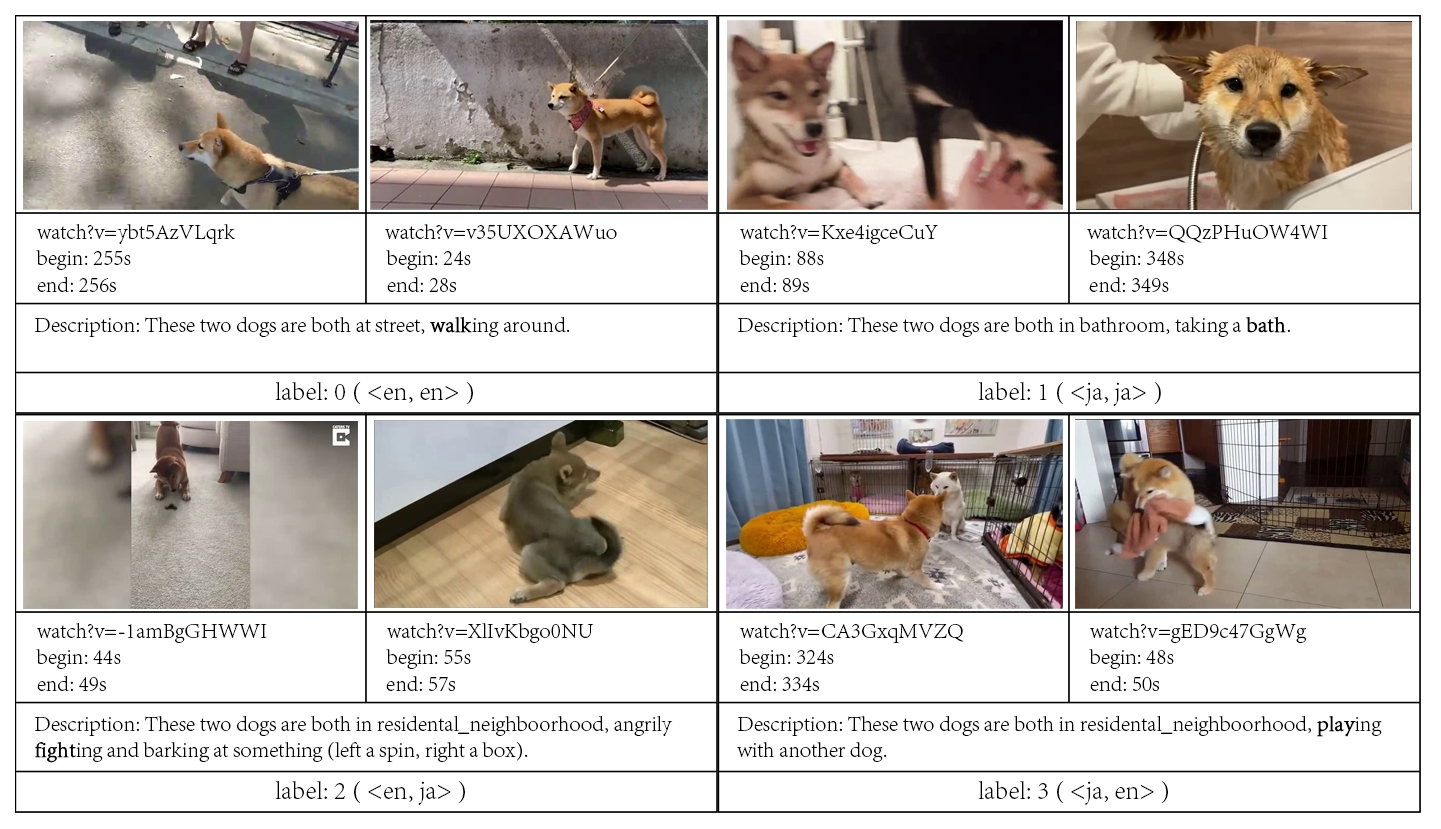
\includegraphics{datasample.png}}
	\caption{Examples from the proposed EJShibaVoice dataset.}
	\label{fig:EJShiba}
\end{figure}

\subsection{Host Speech Extraction}
%\MYW{1 sentence to explain why we care about hosts' language.}
In the second research question of finding the correlation between the barks and their host languages, a dataset of hosts' speech is required. The speech in the original audio track is also extracted by a strict pipeline. The first few steps are similar to dog barking extraction: we start by getting those continuous segments tagging as speech by PANNs and remove those tagged as music from them to reduce the noises.

As there are usually situations when several people are talking together, we apply a speaker diarization model Pyannote\cite{Bredin2020, Bredin2021} to get speech of a single person in smaller grains.

% \KZ{This fig has no ref in the text?}
